\documentclass[margin,line]{resume}

\usepackage[utf8]{inputenc}
\usepackage[english,russian]{babel}
\usepackage[T1]{fontenc}
\usepackage{fontawesome}

% TODO: добавить схему микросервсиной архитектуры с хакатона как пруф
% TODO: сделать автовыраваниване для фотки
% TODO: возможно весь технический скилл написать?
% TODO: сплющить проекты с одинаковым стеком технологий
% TODO: про стартап нписать, поговорить с Марком чтоб его заопенсорсить

\begin{document}

{\sc \large Гришин Антон --- Backend разработчик} \\
\begin{resume}
  \begin{minipage}[t]{0.55\textwidth}
    \section{\mysidestyle Персональная\\Информация}
    Гришин Антон \\
    Москва, Россия \\
    \faGithub  \space
    \href{https://github.com/alchemmist/}{\texttt{alchemmist}} \\
    \faLinkedin \space
    \href{https://www.linkedin.com/in/anton-grishin-6966a8362/}{\texttt{anton-grishin}}
    \\
    \faPaperPlane \space \href{https://t.me/alchemmist}{\texttt{@alchemmist}} \\
    \faPhone \space
    \href{tel:+1234567890}{\color{blue}\texttt{+7(915)067-2638}}  \\
    \faEnvelope \space
    \href{mailto:anton.ingrish@gmail.com}{\color{blue}\texttt{anton.ingrish@gmail.com}}
  \end{minipage}

  \begin{minipage}[H]{0.18\textwidth}
    \begin{textblock}{7}(10.84, 1.7)
      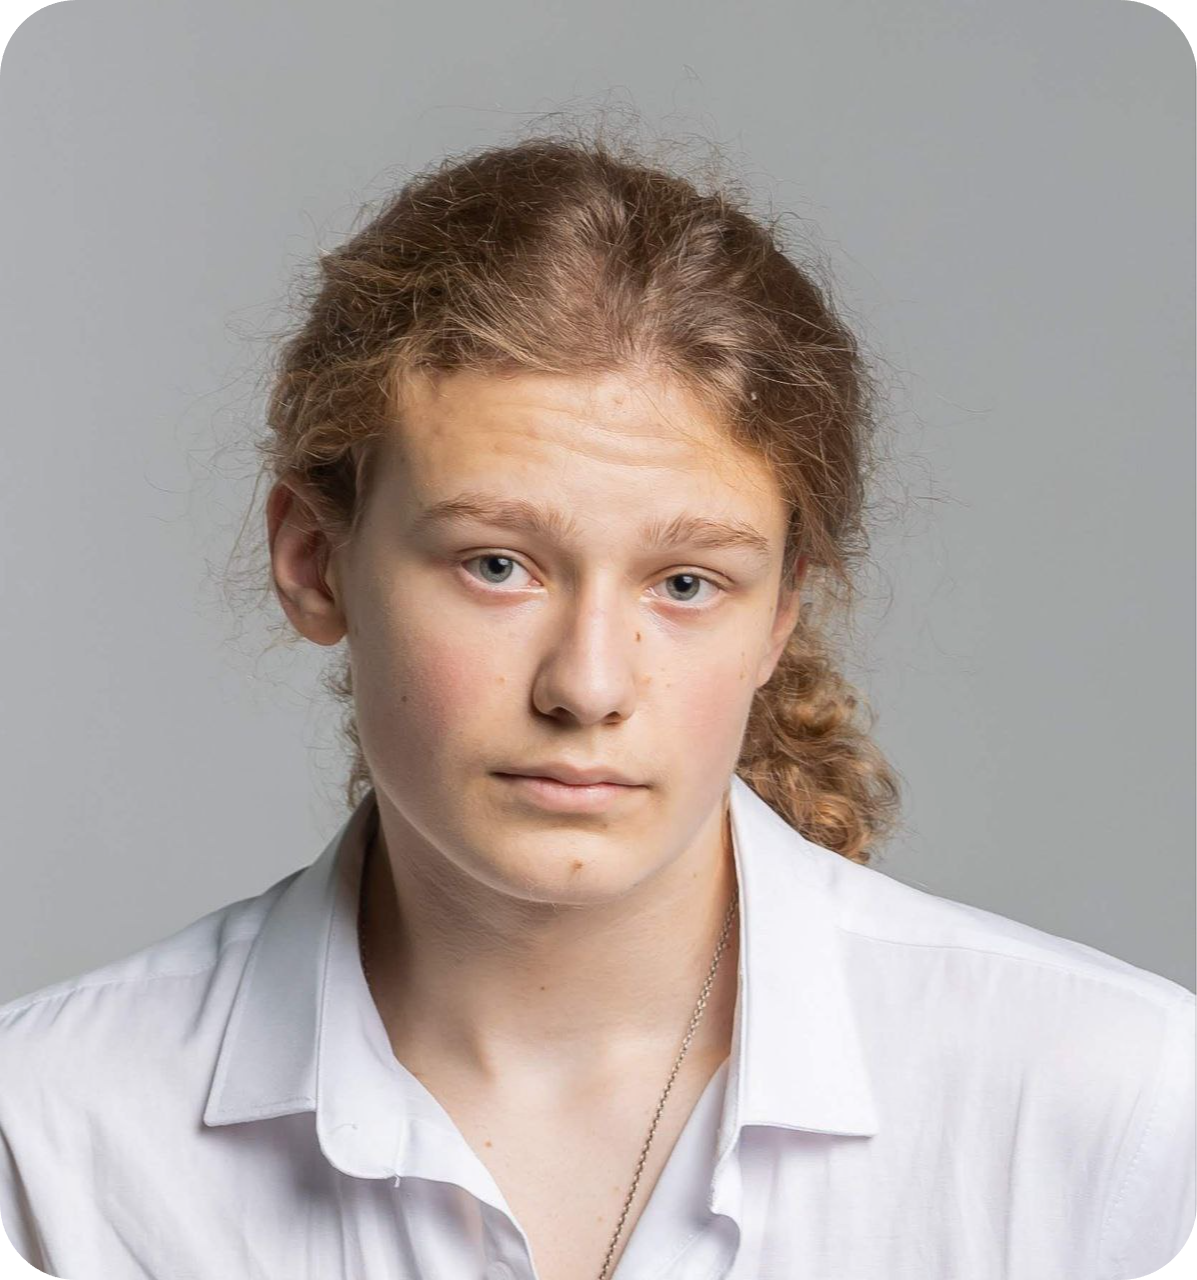
\includegraphics[width=0.27\textwidth]{images/avatar.png}
    \end{textblock}
  \end{minipage}

  \vspace{-5mm}
  \section{\mysidestyle Обо мне}
  Я студент, начинающий разрботчик. Я программирую 4 года; за
  это время я участвовал в разработке 44 репозиториев, отправил 921
  комитов и написал
  176729 строчек кода. В прошлом профессиональный
  \href{https://github.com/alchemmist/CV/blob/main/attachments/sport.pdf}{волейболист}.

  \section{\mysidestyle Навыки}

  \vspace{0.5mm}

  \begin{description}[leftmargin=0pt, itemindent=*]
    \item[Python:] \hangindent=9mm \hangafter=1
      \inlinecode{FastAPI}, \inlinecode{pydantic},
      \inlinecode{Flask},
      \inlinecode{SqlAlchemy}, \inlinecode{faststream},
      \inlinecode{alembic}, \inlinecode{pytest}.
    \item[Go:] \inlinecode{http}, \inlinecode{grpc},
      \inlinecode{protobuf}, \inlinecode{tgbotapi},
      \inlinecode{reflect}, \inlinecode{gofsm}.
    \item[Databases:] \inlinecode{postgres}, \inlinecode{sqlite},
      \inlinecode{redis}, \inlinecode{Yandex Object Storage}.
    \item[Message brokers:] \inlinecode{RebbitMQ}, \inlinecode{Mosquitto}.
    \item[Other techonologies:] \inlinecode{SQL}, \inlinecode{Java},
      \inlinecode{JavaScript}, \inlinecode{bash}.
    \item[Dev tools:] \inlinecode{Docker}, \inlinecode{Podman},
      \inlinecode{Make}, \inlinecode{CI/CD}, \inlinecode{Linux},
      \inlinecode{Git}
    \item[Языки:] Russian, English.
  \end{description}

  \section{\mysidestyle Образование}
  \href{https://centraluniversity.ru/}{Центральный Университет} -
  Математика и компьютерные науки, 2028

  \section{\mysidestyle Cертификаты}
  \textbf{Яндекс Лицей}. Экстерном поступил на второй курс
  \href{https://lyceum.yandex.ru/}{Лицея
  Академии Яндекси} по Промышленной разработке и окончил его с
  \href{https://github.com/alchemmist/CV/blob/main/attachments/yandex-lyceum.pdf}{аттестатом
  с отличием}, сдав финальный проект на 100/100 баллов.

  \vspace{-6mm}

  \hfill \textsl{Сентябрь 2022 - Апрель 2023}

  \textbf{Курс Python}. Прошёл курс по Python на Stepik и завершил его с
  \href{https://github.com/alchemmist/CV/blob/main/attachments/stepik-python-course.pdf}{отличием}.

  \vspace{-3mm}

  \hfill \textsl{Сентябрь 2021 - Апрель 2022}

  \section{\mysidestyle Достижения}
  Прошёл в
  \textbf{\href{https://github.com/alchemmist/CV/blob/main/attachments/russian-chemp-final.pdf}{финал}
    Чемпионата России по спортивному
  программированию,} где разработал
  \href{https://github.com/alchemmist/CV/blob/main/attachments/architect.pdf}{микросервисную
  архитектуру} для
  \href{https://github.com/alchemmist/sportporg}{веб-приложения},
  агрегирующего спортивные события по
  всей России. И разработал алгоритм обработки и проверки ежегодных
  государственных
  отчетов о спортивных мероприятиях. Технический стек:
  \inlinecode{Kafka}, \inlinecode{React}, \\
  \inlinecode{RabbitMQ (FastStream)},
  \inlinecode{FastAPI},
\inlinecode{OAuth}).
% TODO: вложить хакатон на github и добавить ссылку

\vspace{-6mm}

\hfill \textsl{Декабрь 2024}

Я
\textbf{\href{https://github.com/alchemmist/CV/blob/main/attachments/scince-for-life-win.pdf}{победитель}
научно-практической конференции}
«\href{https://conf.profil.mos.ru/academ}{Наука для
жизни}» с \href{https://github.com/smart-cab/}{проектом умного
дома} для частных и государственных
образовательных учреждений. Технический стек: \inlinecode{Redis},
\inlinecode{Zigbee2MQTT}, \inlinecode{websockets}, \inlinecode{Go},
\inlinecode{Python}, \inlinecode{Flask}, \inlinecode{React}.
\vspace{-6mm}

\hfill \textsl{Апрель 2024}

\textbf{Учстник хакаотна \href{https://nuclearhack.mephi.ru/}{Nuclear
IT hack}}, где моя команда работала
над кейсом Росатома: сервис для определения эмоционального тона онлайн-встреч.

\vspace{-6mm}

\hfill \textsl{Апрель 2024}

\textbf{\href{https://github.com/alchemmist/CV/blob/main/attachments/informatics-olimpic.pdf}{Призёр}
3-й степени}, олимпиады МПГУ по информатике:
«Прикладная информатика»
\vspace{-3mm}

\hfill \textsl{Июнь 2023}

\section{\mysidestyle Интересы}\vspace{1mm}
\begin{description}
  \item[Формальная верификация:] Прохожу курс
    \texttt{\href{https://softwarefoundations.cis.upenn.edu}{softwarefoundations}}
    на \inlinecode{Coq}.
  \item[Linux:] Arch, Hyprland
\end{description}
\vfill
% ------------------------------------------------------------------ %

\section{\mysidestyle Петпроекты}\vspace{2mm}

\begin{description}

  \item[SmartCab]\small{\href{https://github.com/smart-cab}{Система
      умного дома} \hfill
    \textsl{Сентябрь 2023 — Май 2024\vspace{2mm}}}\\
    Разработал
    \href{https://www.figma.com/design/8H1tFpxgmIDV1xp06ndi73/SmartCab?node-id=0-1&p=f}{протопипы}
    дизайна админ панели и интерфейса планшета управления
    (\textit{т.н. хаба}). Сверстал их
    (\texttt{\href{https://github.com/smart-cab/smartcab-hub/tree/main/frontend/src}{1}},
    \texttt{\href{https://github.com/smart-cab/smartcab-dashboard/tree/main/frontend/src}{2}})
    на \inlinecode{React}.
    \href{https://github.com/smart-cab/smartcab-bot}{Написал бота}
    для администрирования системы.
    \href{https://github.com/smart-cab/smartcab-hub/blob/main/backend/smartcab/interface/mqtt.py}{Реализовал}
    взаимодействие с умными устройствами по протокулу Zigbee, через
    брокер сообщений Mosquitto.

    Технический стек:
    \begin{list2}
    \item{Язык: \inlinecode{Python}, \inlinecode{Go},
      \inlinecode{JavaScript}, \inlinecode{bash}}
    \item{Фроеймворки: \inlinecode{Flask}}
    \item{Базы данных: \inlinecode{sqlite}, \inlinecode{redis},
      \inlinecode{postgres}}
    \end{list2}
    \vspace{3mm}

  \item[Starship]\small{\href{https://github.com/starship-crew}{Текстовая
      экшн игра в Telegram}
    \hfill \textsl{Март 2023 — Апрель 2023\vspace{2mm}}}\\
    Разработал мехнику
    \href{https://github.com/starship-crew/telegram-client/blob/main/app/handlers/fight.py}{онлайн
    дуэлей} с реальными игроками в Telegram боте. А
    так же удобный
    \href{https://github.com/starship-crew/telegram-client/blob/main/app/template.py}{движок
    рендеринга}
    сообщений в чате через jinja2 шаблоны, так как для тектовой игры
    требовалось гибко работоать с большим количеством сценарных и
    пейзжаных текстов.

    Технический стек:
    \begin{list2}
    \item{Язык: \inlinecode{Python}}
    \item{Библиотеки: \inlinecode{Flask}, \inlinecode{alembic},
        \inlinecode{python-telegram-bot}, \inlinecode{SqlAlchemy},
      \inlinecode{jinja2}}
    \item{Контейнеризация: \inlinecode{Docker}}
    \end{list2}

    \vspace{3mm}

  \item[Corpse]\small{\href{https://github.com/corpse-inc/corpse}{Игровой
      движок}
    \hfill \textsl{Ноябрь 2022 — Январь 2023\vspace{2mm}}}\\
    В команде разработали полнофункциональный модульный
    игровой движок с архитектурой
    \href{https://en.wikipedia.org/wiki/Entity_component_system#:~:text=Entity%E2%80%93component%E2%80%93system%20(ECS,Entity%E2%80%93Component%E2%80%93System%20layout.}{ECS}.
      А так же survival top-down шутер игру о зомбиапокалипсисе.

      Технический стек:
      \begin{list2}
      \item{Язык: \inlinecode{Python}}
      \item{Фреймворк: \inlinecode{Pygame}}
      \item{Библиотеки: \inlinecode{esper}, \inlinecode{pytmx}}
      \item{Инструменты работы с графикой: \inlinecode{aseprite},
        \inlinecode{Tiled}}
      \end{list2}

      \vspace{3mm}

    \item[SchoolRing]\small{\href{https://github.com/alchemmist/school-ring}{Управление
        звонками в школах}
        \begingroup
        \hypersetup{urlcolor=blue!30}
        \href{https://github.com/}{\texttt{release v0.0.2}}
        \endgroup
        \hfill
      \textsl{Октябрь 2022 — Ноябрь 2022\vspace{2mm}}}\\
      Настроил
      \href{https://github.com}{\texttt{pre-commit}} для
      амтоматической конвертации \inlinecode{.ui} файлов в
      \inlinecode{.py}, а так же \href{https://github.com}{Github
      Actions} для автоматической сборки нового релиза под все
      операционные системы при каждом комите в main. Недавно перевол
      проект на \href{https://astral.sh/blog/uv}{\texttt{uv}} для
      удобного управления зависимостями.
      % TODO: сделать рабочий релиз
      % TODO: настроить pre-commit для .ui -> .py (написать об этом здесь)
      % TODO: перехать только на pyqt6
      % TODO: настроить pre-commit и добавить ссылку на файл
      % TODO: подконец исправить версию релиза

      Технический стек:
      \begin{list2}
      \item{Язык: \inlinecode{Python}}
      \item{Фреймворк: \inlinecode{PyQt6}}
      \item{Стандартная библиотека: \inlinecode{threading},
        \inlinecode{schedule}}
      \end{list2}

  \end{description}

  \section{\mysidestyle Заказная разработка}\vspace{2mm}

  \begin{description}

    \item[SmartCab]\small{\href{https://github.com/smart-cab}{Система
        умного дома} \hfill
      \textsl{Сентябрь 2023 — Май 2024\vspace{2mm}}}\\
      Разработал
      \href{https://www.figma.com/design/8H1tFpxgmIDV1xp06ndi73/SmartCab?node-id=0-1&p=f}{протопипы}
      дизайна админ панели и интерфейса планшета управления
      (\textit{т.н. хаба}). Сверстал их
      (\texttt{\href{https://github.com/smart-cab/smartcab-hub/tree/main/frontend/src}{1}},
      \texttt{\href{https://github.com/smart-cab/smartcab-dashboard/tree/main/frontend/src}{2}})
      на \inlinecode{React}.
      \href{https://github.com/smart-cab/smartcab-bot}{Написал бота}
      для администрирования системы.
      \href{https://github.com/smart-cab/smartcab-hub/blob/main/backend/smartcab/interface/mqtt.py}{Реализовал}
      взаимодействие с умными устройствами по протокулу Zigbee, через
      брокер сообщений Mosquitto.

      Технический стек:
      \begin{list2}
      \item{Язык: \inlinecode{Python}, \inlinecode{Go}}
      \end{list2}
      \vspace{3mm}

  \end{description}
\end{resume}
\end{document}
